%\documentclass{llncs}
\documentclass{llncs} %[runningheads] for title-header on every page



\typeout{}
\typeout{--------------------------------------------------------------}
\typeout{ +---+ Thesis Template                            }
\typeout{ +---+      Version 2.0, August 2011                         }
\typeout{ +---+  for Instituto Superior Tecnico (IST),                 }
\typeout{ +---+  Universidade T�cnica de Lisboa                         }
\typeout{ * Using Thesis Style form Pedro Tom�s                                }
\typeout{ * Created to write Dissertations                             }
\typeout{ * Conforms with IST Master Degree format and with most important packages setup        }
\typeout{ * Should conform with IST PhD Degree format (not verified)   }
\typeout{                                                              }
\typeout{ AUTHOR: Miguel Amador and Jo�o Marques                                          }
\typeout{                                                              }
\typeout{Important: Use all files in the archive, since this is based in all them. Modify dummy files at wish.                                                              }
\typeout{--------------------------------------------------------------}
\typeout{}

% Defines an additional alphabet... not required in most cases
% ------------------------------------------------------------
% \DeclareMathAlphabet{\mathpzc}{OT1}{pzc}{m}{it}

% PACKAGE babel:
% ---------------
% The 'babel' package may correct some hyphenisation issues of latex. 
% However in most situations it is not required.
\usepackage[english]{babel}

% PACKAGE fontenc:
% -----------------
% chooses T1-fonts and allows correct automatic hyphenation.
%\usepackage[T1]{fontenc}
\usepackage[latin1]{inputenc}
%\usepackage[utf8]{inPUTenc}									% UTF 8, Caracteres ocidentais

% PACKAGE eurosym:
% -----------------
% allows the use of the european currency sign
\usepackage{eurosym}

% PACKAGE lettrine:
% -----------------
% allows the use of drop cap lettering
\usepackage{type1cm}
\usepackage{lettrine}

% Package ulem.
\usepackage{ulem} % Allows the use of other text emphatizer commands
\normalem %defines \emph{} to italic, instead of underline. 
\raggedbottom %declaration makes all pages the height of the text on that page. No extra vertical space is added. The \flushbottom declaration makes all text pages the same height, adding extra vertical space when necessary to fill out the page.

% PACKAGE date time:
% -----------------
% Lets you alter the format of the date that \today returns.
\usepackage{datetime}
\newdateformat{todaythesis}{%
\monthname[\THEMONTH]  \THEYEAR}

% PACKAGE latexsym:
% -----------------
% Defines additional latex symbols. May be required for thesis with many math symbols.
\usepackage{latexsym}

% PACKAGE amsmath, amsthm, amssymb, amsfonts:
% -------------------------------------------
% This package is typically required. Among many other things it adds the possibility
% to put symbols in bold by using \boldsymbol (not \mathbf); defines additional 
% fonts and symbols; adds the \eqref command for citing equations. I prefer the style
% "(x.xx)" for referering to an equation than to use "equation x.xx".
\usepackage{amsmath, amsthm, amssymb, amsfonts, amsbsy}

% PACKAGE multirow, colortbl, longtable:
% ---------------------------------------
% These packages are most useful for advanced tables. The first allows to join rows 
% through the command \multirow which works similarly with the command \multicolumn
% The second package allows to color the table (both foreground and background)
% The third package is only required when tables extend beyond the length of one page;
% with compatibilities with the tabular environment. The last allow the definitions of landscape pages, allowing the use of a different orientation for wider graphics or tables. See package documentation to see the implementation.
\usepackage{multirow}
\usepackage{colortbl}
\usepackage{supertabular}
\usepackage{pdflscape}
% \usepackage{longtable}

% PACKAGE graphics, epsfig, subfigure, caption:
% ---------------------------------------------
% Packages for figures... well you will certainly need these packages, with the exception
% of the 'caption' package. This only allows to define extra caption options.
% Notice that subfigure allows to place figures within figures with its own caption. It
% should be avoided to create an eps file with subfigures. That will mean that you won't be 
% able to reference those subfigures. Instead create an EPS file (the only graphics format supported
% by latex) for each of the subfigures and then use the command \subfigure (see below).
\usepackage{graphics}
\usepackage{graphicx}
\usepackage{epsfig}
\usepackage[hang,small,bf]{subfigure}
%\usepackage[footnotesize,bf,center]{caption}
\usepackage{dcolumn}
\usepackage{bm}
\usepackage{booktabs}
\usepackage{rotating}
\usepackage{multirow}

\usepackage[font=small,labelfont=bf,textfont=normalfont]{caption}

% PACKAGE algorithmic, algorithm
% ------------------------------
% These packages are required if you need to describe an algorithm.
% \usepackage{algorithmic}
% \usepackage[chapter]{algorithm}

% PACKAGE natbib/cite
% -------------------
% The two packages are not compatible, and you should use one of the two. Notice however that the
% IEEE BiBTeX stylesheet is imcompatible with the natbib package. If using the IEEE format, use the 
% cite package instead
%\usepackage[square,numbers,sort&compress]{natbib}
\usepackage{cite}

% PACKAGE acronym
% -----------------
% This package is most useful for acronyms. The package guarantees that all acronyms definitions are 
% given at the first usage. IMPORTANT: do not use acronyms in titles/captions; otherwise the definition 
% will appear on the table of contents.
\usepackage[printonlyused]{acronym}
\usepackage[titletoc,title,header]{appendix}
\usepackage[noauto]{chappg}

% PACKAGE extra_functions
% -----------------
% My Personal package: defines the following commands:
% \fancychapter{chaptername) -> Prints a fancier chapter (you can also use the fancychapter package for this)
% \hline{width} -> use for a replacement of the \hline command
% \Mark1, \Mark2, \Mark3, ...
\usepackage{00.extra_functions}


% PACKAGE hyperref
% -----------------
% Set links for references and citations in document
% Some MiKTeX distributions have faulty PDF creators in which case this package will not work correctly
% Long live Linux :D
\usepackage[plainpages=false]{hyperref}
\hypersetup{
             colorlinks=false,
             citecolor=red,
             breaklinks=true,
             bookmarksnumbered=true,
             bookmarksopen=true,
             pdftitle={Benchmark Kinect},
             pdfauthor={Jo�o Pedro Ribeiro Machado},
             pdfsubject={Master Thesis in Information Systems and Computer Engineering},
             pdfcreator={TeXstudio},
             pdfkeywords={Template, Latex, Thesis}}
\usepackage{float}
%\usepackage[final]{00.listofsymbols}
\usepackage{00.symlist}

% Set paragraph counter to alphanumeric mode
\renewcommand{\theparagraph}{\Alph{paragraph}~--}

\newcommand{\figref}[1]{Figure \ref{#1}}
\newcommand{\equationref}[1]{Equation (\ref{#1})}
\newcommand{\tableref}[1]{Table (\ref{#1})}

\newcommand{\textreg}{$\textsuperscript{\textregistered}$}


% MINE MINE
\newcounter{eqn}
\renewcommand*{\theeqn}{\alph{eqn})}
\newcommand{\num}{\refstepcounter{eqn}\text{\theeqn}\;}

\makeatletter
\newcommand{\putindeepbox}[2][0.7\baselineskip]{{%
    \setbox0=\hbox{#2}%
    \setbox0=\vbox{\noindent\hsize=\wd0\unhbox0}
    \@tempdima=\dp0
    \advance\@tempdima by \ht0
    \advance\@tempdima by -#1\relax
    \dp0=\@tempdima
    \ht0=#1\relax
    \box0
}}
\makeatother


% MINE MINE



% load package with ``framed'' and ``numbered'' option.
\usepackage[framed,numbered,autolinebreaks,useliterate]{mcode}

% something NOT relevant to the usage of the package.
\setlength{\parindent}{0pt}
\setlength{\parskip}{18pt}
\title{\texttt{mcode.sty} Demo}
\author{Florian Knorn, \texttt{florian@knorn.org}}
% //////////////////////////////////////////////////
\begin{document}
{\bf List of Abreviations:}
\begin{acronym}
 

\acro{CPT}[CPT]{Conditional Probability Table}
\acro{DAG}[DAG]{Directed Acyclic Graph} 
\acro{DBN}[DBN]{Dynamic Bayesian Networks}
\acro{HMM}[HMM]{Hidden Markov Models}
\acro{QBN}[QBN]{Quantum Bayesian Networks} 
\end{acronym}


\subsubsection{Hidden Markov Models}
\ac{HMM} are a temporal statistical tool, known as Markov Model, which allows representing systems where we have a hidden layer and an output layer, that depends on the hidden layer\cite{eemcs5901}\cite{Norvig2003}. An example of a simple Markov Model could be a Markov Chain. However Markov Chains don’t have hidden layers because the state of the system is completely visible to the observer; in the roulette example (Figure \ref{fig:roulette}), we know at each moment which if we have a red house. 

In \ac{HMM}, the hidden states are not directly visible, only the output is visible\cite{citeulike:405907}. So, in order to predict the current state of the hidden layer we take into account past outputs. 

\subsubsection{Dynamic Bayesian Networks}
\ac{DBN}, also known as Two-Timeslice Bayesian Networks, are an extension of the common Bayesian Network to deal with a temporal evolution\cite{eemcs5901}. \ac{DBN} have resemblances to \ac{HMM}. More accurately we can say that \ac{HMM} are special cases of \ac{DBN}, a \ac{DBN} single discrete state variable\cite{Norvig2003}. 

The temporal dimension in \ac{DBN} is represented as time-steps. Each time step corresponds to a classical Bayesian Network, but the nodes in this Bayesian Network can have temporal links, represented as a directed edge to the next time-step, this means that these nodes will have influence on the variables of the nodes they connect with, in the following time-step.

\begin{figure}[h]
\centering 

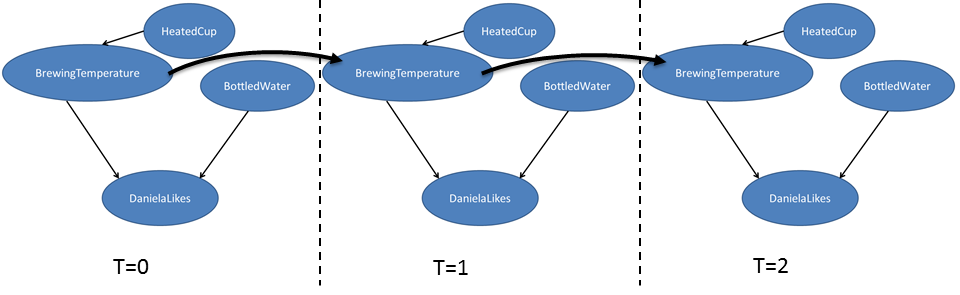
\includegraphics[scale=0.48]{Overview/Figures/TeaPreparationNetworkDBN.png}
\caption{Time evolution of the ``Tea preparation network".}
\label{fig:tea_networkdbn}
\end{figure}

In the Figure \ref{fig:tea_networkdbn} we have a possible transformation of the example of the ``Tea Preparation" to accommodate a time evolution. The variable Brewing Temperature at a given time-step will depend on the brewing temperature in the previous measurement (empiricaly we know that the temperature will not increase given the last time-step). 


\section{Proposal}
As the theory behind Quantum Mechanics evolved in order to explain phenomena that could not be explained merely by classical Physics, Quantum Cognition resorts to the same mathematical foundations in order to explain cognitive phenomena (Section \ref{subsec:QuantumCog}). 

The fact that our beliefs may not be correctly explained or expressed by classical probabilistic frameworks when there's uncertainty involved may suggest that these frameworks could be incomplete. Furthermore there's empirical evidence that von Neumann probabilities may be used to represent Human beliefs with more accuracy than the classical probabilities\cite{Busemeyer2011}\cite{Busemeyer2009423}. Moreover the von Neumann probabilities enable simpler explanations for known paradoxes and falacies in Human judgements. Thus the investigation of the hypothesis of using quantum probabilities to replace classical bayesian probabilities in a popular framework, such as the Bayesian Networks, may hold interesting results, in term of accuracy. 

This study will be centered on the analisys of the usage of von Neumann probabilities in Bayesian Networks. The Bayesian Networks were initialy proposed\cite{Pearl1985} as a tool that could model the way Humans construct their knowledge. Nowadays they've become ubiquitous and are used in areas such as medical diagnosis, weather forecast, speech recognition, etc... 

We will investigate if the usage of Quantum Probabilities in Bayesian Networks has any advantage over the classical setting. When making this comparrison we need to take into account that the classical system is equivalent to the quantum system if we ``measure" the result at each step (Section \ref{subsec:relation}). 

To compare the classical setting and the quantum setting, first we will replace the classical probabilities in a thourougly known Bayesian Network such as the ``burglary network"\cite{Pearl1988}, presented in Section \ref{subsec:int_BN}. To test and compare the quantum approach and the classical approach, empirical evaluation of the data will be made. After modeling a simpler Bayesian Network with quantum probabilities we plan to extend the idea to a more complex Bayesian Network. For this step we will use an existing dataset on Bayesian Networks\footnote{ Bayesian Network Repository: \url{http://www.cs.huji.ac.il/site/labs/compbio/Repository/}}. This will allow an empirical evaluation of the Quantum approach and a better reproducibility of our experiment as well. The main objective is to compare whether or not the Bayesian Networks using quantum probabilities achieve more accurate results when modeling human behaviour. 

Although some there is already some work in which quantum probabilities are applied to Bayesian Networks (Section \ref{subsec:int_QBN}), this proposal tries to capture that idea and transpose it to the Quantum Cognition Domain. Also, if possible we will try to extend our research to \ac{HMM} and consequentially to \ac{DBN}. Considering the time evolution of the system is an interesting topic to explore in the domain of Quantum Cognition, as our beliefs change over time but at the same time our mind tries to create a continuum to help with our self-regulation\cite{RefWorks:61}.

The development of the prototype will be implemented in MATLAB. This numerical environment was chosen as a prototyping tool due to its built-in tools that allow for matrix manipulation, which will be thoroughly used. Moreover there is already some academic work on Quantum Cognition developed in this framework\cite{Busemeyer2009423}\cite{Trueblood}\cite{Busemeyer2009}\cite{Busemeyer:2012:QMC:2385442}. There is also a support for Bayesian Networks in Matlab, by using the ``Bayes Net Toolbox"\footnote{Bayes Net Toolbox: \url{https://code.google.com/p/bnt/}} which implements algorithms for inference and learning. When comparing this toolbox with other existing frameworks also meant to work with Bayesian Networks we find that the ``Bayes Net Toolbox” doesn’t support a graphical user interface (GUI). On other hand the ``Bayes Net Toolbox” for MATLAB is Open Source and supports Dynamic Bayesian Networks and Hidden Markov Models. SamIam\footnote{ SamIam: \url{ http://reasoning.cs.ucla.edu/samiam/}} is a graphical tool that also allows inference in Bayesian Networks and has the advantage of having a GUI. 





%\bibliographystyle{IEEEtran}
\bibliographystyle{splncs}
%\bibliographystyle{ieeetr}
\bibliography{02.biblio}


\begin{comment}
% Table of Contents

% make a proper TOC despite llncs

\setcounter{tocdepth}{2}
\makeatletter
\renewcommand*\l@author[2]{}
\renewcommand*\l@title[2]{}
\makeatletter
\tableofcontents
%
\end{comment}

\end{document}
